
\documentclass{beamer}
\usetheme{Electromagnetism}
\usepackage{Electromagnetism}
\graphicspath{{pictures/}}
% -------------------------------------- Grid
%-------------------------------------------------------
\makeatletter
\def\grd@save@target#1{%
  \def\grd@target{#1}}
\def\grd@save@start#1{%
  \def\grd@start{#1}}
\tikzset{
  grid with coordinates/.style={
    to path={%
      \pgfextra{%
        \edef\grd@@target{(\tikztotarget)}%
        \tikz@scan@one@point\grd@save@target\grd@@target\relax
        \edef\grd@@start{(\tikztostart)}%
        \tikz@scan@one@point\grd@save@start\grd@@start\relax
        \draw[minor help lines] (\tikztostart) grid (\tikztotarget);
        \draw[major help lines] (\tikztostart) grid (\tikztotarget);
        \grd@start
        \pgfmathsetmacro{\grd@xa}{\the\pgf@x/1cm}
        \pgfmathsetmacro{\grd@ya}{\the\pgf@y/1cm}
        \grd@target
        \pgfmathsetmacro{\grd@xb}{\the\pgf@x/1cm}
        \pgfmathsetmacro{\grd@yb}{\the\pgf@y/1cm}
        \pgfmathsetmacro{\grd@xc}{\grd@xa + \pgfkeysvalueof{/tikz/grid with coordinates/major step}}
        \pgfmathsetmacro{\grd@yc}{\grd@ya + \pgfkeysvalueof{/tikz/grid with coordinates/major step}}
        \foreach \x in {\grd@xa,\grd@xc,...,\grd@xb}
        \node[anchor=north] at (\x,\grd@ya) {\pgfmathprintnumber{\x}};
        \foreach \y in {\grd@ya,\grd@yc,...,\grd@yb}
        \node[anchor=east] at (\grd@xa,\y) {\pgfmathprintnumber{\y}};
      }
    }
  },
  minor help lines/.style={
    help lines,
    step=\pgfkeysvalueof{/tikz/grid with coordinates/minor step}
  },
  major help lines/.style={
    help lines,
    line width= 0.5pt,
    step=\pgfkeysvalueof{/tikz/grid with coordinates/major step}
  },
  grid with coordinates/.cd,
  minor step/.initial=.2,
  major step/.initial=1,
  major line width/.initial=2pt,
}
\makeatother
\usepackage{cancel}
\usetikzlibrary{shapes.geometric,calc}


\tikzset{
        custom dash/.style={
            dash pattern=on 2pt off 0.7pt
        }
    }

\begin{document}


% ============================== Слайд ## ===================================
\begin{frame}{Скін-ефект}{Оцінка глибини проникнення поля в провідник}
	%	\begin{onlyenv}<1>
	%		\begin{columns}
	%			\begin{column}{0.3\linewidth}\centering
	%				\begin{tikzpicture}[>=latex]
	%					% Основные параметры
	%					\pgfmathsetmacro\h{3}          % Высота
	%					\pgfmathsetmacro\R{1}          % Радиус
	%					\coordinate (A) at (0, {-\h/2});
	%					\coordinate (B) at (0, {+\h/2});
	%
	%					% Вертикальные линии
	%					\draw[gray] ([xshift=\R cm]A) -- ([xshift=\R cm]B)
	%					([xshift=-\R cm]A) -- ([xshift=-\R cm]B);
	%					\draw[line width={\R*2cm}, gray!50] (A) -- (B);
	%
	%					% Верхняя и нижняя части
	%					\draw[gray, fill=gray!50] (B) circle ({\R} and {0.2*\R});
	%					\draw[gray] ([xshift=\R cm]A) arc(0:-180:{\R} and {0.2*\R});
	%					\draw[gray, densely dashed] ([xshift=-\R cm]A) arc(180:0:{\R} and {0.2*\R});
	%					\fill[gray!50] (A) circle ({\R} and {0.2*\R});
	%
	%					% Стрелка для тока
	%					%    \draw[->] ([yshift={\h*0.3cm}]A) -- ([yshift={-\h*0.3cm}]B) node[above] {$I$};
	%					\draw[green!70!black, thick,
	%						arrowpos={0.15}{2pt}{3pt},
	%						arrowpos={0.40}{2pt}{3pt},
	%						arrowpos={0.70}{2pt}{3pt},
	%						arrowpos={0.90}{2pt}{3pt}
	%					] (-1,-0.5) -- ++(0,1) -- ++(0.5, 0) -- ++(0, -1) -- cycle;
	%
	%					\def\fLarge{0.95}  % Масштаб большого витка
	%
	%					\foreach \x in {0,0.1,...,0.5}{
	%							\draw[->, red, ultra thin] ({\x-1},-0.5) -- ++(0, {1-2*\x});
	%						}
	%
	%					\foreach \y in {-0.4,0,0.4} {
	%					\draw[arrowpos={0.5}{0}{2pt}, blue, ultra thin] (0,{\fLarge*\y})
	%					[partial ellipse=91:{360+89}:{\fLarge*\R} and {\fLarge*0.1*\R}];
	%					}
	%
	%					\node[left, font=\scriptsize, text=red] at (-1, 0.5) {$\Efield$};
	%					\node[below, font=\scriptsize] at (-0.75, -0.5) {$\delta$};
	%					\node[left, font=\scriptsize] at (-1, 0) {$h$};
	%
	%				\end{tikzpicture}
	%			\end{column}
	%			\begin{column}{0.7\linewidth}
	%				\begin{block}{}\justifying
	%					Знайдемо циркуляцію вектора \textcolor{red}{$\Efield$} вздовж контура \textcolor{green!60!black}{$L$}. За законом електромагнітної
	%індукції:
	%					\begin{equation*}
	%						Eh = - \frac1c\frac{\Delta\Phi}{\Delta t}.
	%					\end{equation*}
	%					Магнітний потік через цей контур:
	%					\begin{equation*}
	%						\Phi = -BS = \mu H h \delta.
	%					\end{equation*}
	%					Його зміна за одиницю часу (тобто похідна за часом) буде порядку
	%					\(
	%					\frac{\Delta\Phi}{\Delta t} \approx \frac{\Phi}{T} \approx \omega \Phi,
	%					\)
	%					де $T$ --- період зміни струму, $\omega$ --- частота зміни струму, $\omega \sim \frac1T $.
	%				\end{block}
	%			\end{column}
	%		\end{columns}
	%		\begin{block}{}\justifying
	%			Тому, циркуляція вектора $\Efield$ буде дорівнювати:
	%			\(
	%			E h = \frac1c \mu H\omega h \delta,
	%			\) а величина електричного поля на поверхні провідника:
	%			\begin{equation*}
	%				E = \frac1c \mu H\omega \delta
	%			\end{equation*}
	%		\end{block}
	%	\end{onlyenv}
	%	\begin{onlyenv}<2>
	%		\begin{columns}
	%			\begin{column}{0.3\linewidth}
	%				\begin{tikzpicture}[>=latex]
	%
	%					\draw[gray, fill=gray!50] (0,0) circle(1.5);
	%					%        \draw[arrowpos={0.5}{2pt}{4pt}, blue, ultra thin] circle (1.35);
	%					\draw[green!60!black, thick,
	%						arrowpos={0.15}{2pt}{4pt},
	%						arrowpos={0.4}{2pt}{4pt},
	%						arrowpos={0.7}{2pt}{4pt},
	%						arrowpos={0.85}{2pt}{4pt},
	%					] (-1.5, 0.25) --
	%					node[left, font=\scriptsize, text=black] {$\ell$}
	%					++(0, -0.5) --  node[below, font=\scriptsize, text=black] {$\delta$}
	%					++(0.5, 0) -- ++(0, 0.5) -- cycle;
	%
	%					\foreach[count=\c] \x in {0,0.1,...,0.5}{
	%							\draw[->, blue, ultra thin] ({\x-1.5},0.25) -- ++(0, {-(1-2*\x)})
	%							\ifnum\c=1 node[pos=1, left] {$\Hfield$}\fi;
	%						}
	%					\foreach \a in {0,30,...,330} {
	%							\draw[] (\a:1.25) circle(0.05);
	%							\fill[] (\a:1.25) circle(0.025);
	%							\ifnum\a=90\node[below, font=\scriptsize, red] at (\a:1.3){$\vect{j}$}\fi;
	%						}
	%				\end{tikzpicture}
	%			\end{column}
	%			\begin{column}{0.7\linewidth}
	%				\begin{block}{}\justifying
	%					Тепер знайдемо циркуляцію напруженості
	%					магнітного поля \textcolor{blue}{$\Hfield$} по контуру \textcolor{green!60!black}{$L$}. За теоремою про циркуляцію:
	%					\begin{equation*}
	%						H \ell = \frac{4\pi}{c} j \ell \delta.
	%					\end{equation*}
	%					Так як $j = \lambda E$, і після спрощення знаходимо магнітне поле на поверхні провідника:
	%					\begin{equation*}
	%						H = \frac{4\pi}{c} \lambda E \delta.
	%					\end{equation*}
	%				\end{block}
	%			\end{column}
	%		\end{columns}
	%		\begin{block}{}\justifying
	%			Підставимо величину напруженості магнітного поля у знайдену формулу $E = \frac1c \mu H\omega \delta$:
	%			\begin{equation*}
	%				E =  \frac{4\pi\mu\omega \delta^2}{c^2} \lambda E,
	%			\end{equation*}
	%			Звідки, оцінка глибини проникнення поля дає величину:
	%			\begin{equation*}
	%				\delta = \frac{c}{\sqrt{4\pi\mu\lambda\omega}}.
	%			\end{equation*}
	%		\end{block}
	%	\end{onlyenv}
\end{frame}
% ===========================================================================



% ============================== Слайд ## ===================================
\begin{frame}{Вершина класичної науки}{}\small
	\begin{block}{}\justifying
        \alert{Рівняння Максвелла --- це вершина класичної науки про електромагнітне поле.} До цієї висоти ми піднімалися, крок за кроком, уточнюючи
        поняття і розкриваючи глибинні принципи цієї науки. Кожен пройдений етап — електростатика, закони постійного струму, магнітостатика — був немов
        базовий табір на шляху до вершини.

        \medskip

        На вершині перед нами постають Рівняння Максвелла --- велична симфонія електричного і магнітного полів, ключ до розуміння електромагнітної
        взаємодії. Але шлях науки триває. З вершини ми спускаємося у простір застосувань: досліджуємо поширення електромагнітних хвиль, принципи
        випромінювання та закладаємо основи оптики, радіо- й електротехніки.

        \medskip

        Ця подорож --- не лише тріумф інтелекту, а й людського духу, що прагне підкорювати вершини й відкривати нові горизонти.
	\end{block}
	\begin{center}
        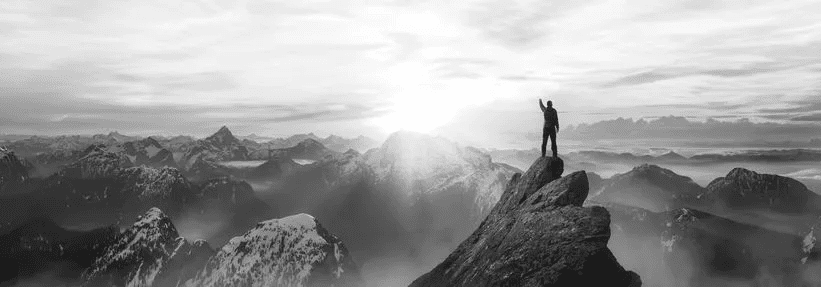
\includegraphics[height=3cm]{ontop}
	\end{center}
\end{frame}
% ===========================================================================


\end{document}